% Required packages (if not already in preamble):
%   \usepackage{graphicx, booktabs, subcaption, amsmath}
% Figures are in paper_materials/figs/

\section{Further Investigation on Cross-Domain Calibration Performance}
\label{sec:cross_domain_investigation}

Table~\ref{tab:cross-domain-calibration} contains an apparent anomaly: for MMLU as the
test domain, cross-domain calibrators trained on SQuAD~2.0 and TruthfulQA achieve
\emph{larger} reductions in faithfulness divergence than the in-domain MMLU calibrator,
despite having no access to in-distribution data.
We attribute this to a weak in-domain calibration signal unique to MMLU, amplified by
a shared overconfidence direction across all three datasets.

MMLU exhibits an anomalously small overconfidence bias: the gap between mean confidence
and mean accuracy is only $0.049$ for linguistic confidence, compared to $0.285$ and
$0.360$ for SQuAD~2.0 and TruthfulQA respectively (Table~\ref{tab:bias};
Figure~\ref{fig:bias}).
With such a small target signal and only $4{,}212$ training samples drawn from
57 heterogeneous subjects, the in-domain calibrator fits a near-flat reliability curve
and cannot learn a reliable correction.
This instability is evident in the high variance of the in-domain MMLU improvement
($\pm 0.18$) in Table~\ref{tab:cross-domain-calibration}.
Cross-domain sources with strong, consistent overconfidence produce calibrators
that learn a reliable downward correction; because all three datasets share the same
overconfidence direction, this correction transfers to MMLU even though its magnitude
differs.

\begin{figure}[t]
  \centering
  \begin{subfigure}[b]{0.48\linewidth}
    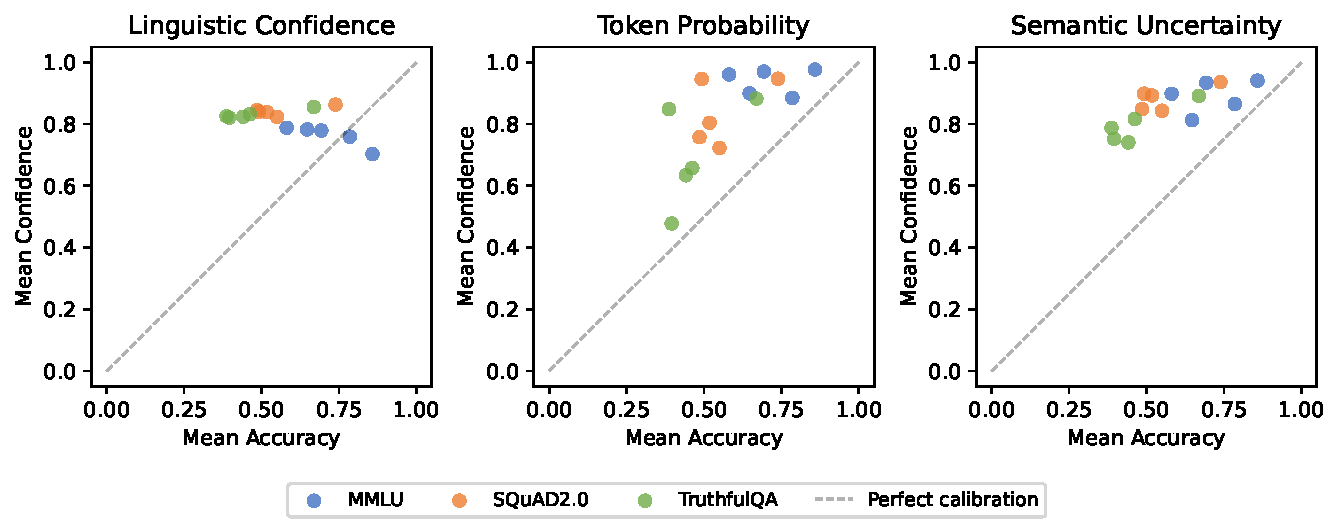
\includegraphics[width=\linewidth]{figs/h2_miscalibration_bias.pdf}
    \caption{Mean confidence vs.\ mean accuracy per (dataset, model) pair.
             All datasets are overconfident (above the diagonal), but MMLU's
             bias is substantially smaller.}
    \label{fig:bias}
  \end{subfigure}
  \hfill
  \begin{subfigure}[b]{0.48\linewidth}
    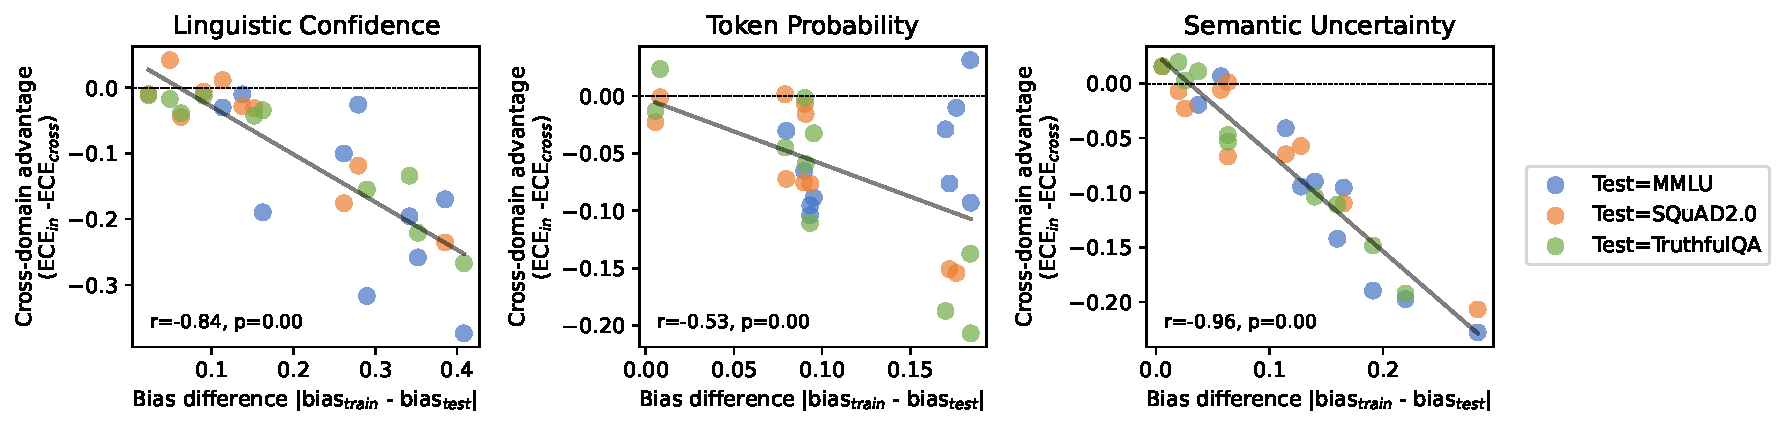
\includegraphics[width=\linewidth]{figs/h2_bias_vs_advantage.pdf}
    \caption{Overconfidence bias difference $|\bar{b}_\text{train} - \bar{b}_\text{test}|$
             vs.\ cross-domain advantage.
             Colour indicates the test dataset.}
    \label{fig:bias_corr}
  \end{subfigure}
  \caption{
    Overconfidence bias per dataset (left) and its relationship to cross-domain
    calibration advantage (right; $r = -0.814$, $p < 0.001$).
    When source and target domains share a similar bias, cross-domain performance
    approaches in-domain performance; when biases diverge, in-domain calibration
    recovers its advantage -- except when the in-domain signal is itself too weak
    to be reliable, as is the case for MMLU.
  }
  \label{fig:bias_combined}
\end{figure}

\begin{table}[h]
  \centering
  \small
  \caption{Mean overconfidence bias (mean confidence $-$ mean accuracy)
           per dataset and confidence signal, averaged over models.}
  \label{tab:bias}
  \begin{tabular}{lccc}
    \toprule
    Dataset        & Ling.\ Conf. & Token Prob. & Sem.\ Unc. \\
    \midrule
    MMLU           & $0.049$      & $0.225$     & $0.177$    \\
    SQuAD~2.0      & $0.285$      & $0.278$     & $0.326$    \\
    TruthfulQA     & $0.360$      & $0.229$     & $0.326$    \\
    \bottomrule
  \end{tabular}
\end{table}

We quantify this mechanism by correlating the overconfidence bias difference
$|\bar{b}_\text{train} - \bar{b}_\text{test}|$ with the cross-domain advantage
(Figure~\ref{fig:bias_corr}).
We observe a strong negative relationship ($r = -0.814$, $\rho = -0.786$,
$p < 0.001$): transfer pairs whose source and target exhibit similar overconfidence
biases show smaller performance gaps, whereas dissimilar biases favour in-domain
calibration.
Accuracy-level alignment between source and target provides a complementary signal
($r = -0.765$, $p < 0.001$): when the two domains have similar mean accuracy rates,
the learned correction maps confidences into an appropriate range for the target domain,
facilitating transfer.
Together, these findings indicate that cross-domain calibration is most effective when
the source domain provides a stronger and more reliable overconfidence signal than
the target domain's own in-distribution data, and when the two domains share a
similar accuracy level.
